\documentclass[11pt,a4paper]{article}

\usepackage[margin=2.5cm]{geometry}
\usepackage{graphicx}
\usepackage{subcaption}
\usepackage{amsmath}
\usepackage{amssymb}
\usepackage{booktabs}
\usepackage{xcolor}
\usepackage{hyperref}
\hypersetup{colorlinks=true, linkcolor=blue, urlcolor=blue, citecolor=blue}

\graphicspath{{figures/}}

\title{Final project: Learning a Value Function with a Neural Network,\\
and Using it as Terminal Cost in an Optimal Control Problem}
\author{Alessandro Wegher \\ n.m. 249819}
\date{University of Trento \\ Department of Industrial Engineering \\ Via Sommarive 14, 38123 Povo (TN), Italy}

\begin{document}
\maketitle

\section{Introduction}

Solving OCPs over long time horizons can be computationally very expensive and introduce
quite high latency in real-time control of a robotic system. To improve the performance of
the optimal-trajectory computation, we can rely on a model that approximates the function
relating the initial state of the MPC $x(t_k)$ to the cost we would obtain by going optimally
to the final state at the end of the horizon $x(t_k + N \cdot T_s)$.

In order to address this challenge, we train a simple neural network as a function-approximation
structure that takes the initial state of the MPC $x_0$ as input and approximates the value of
the terminal cost function $V_{nn}(x_0, N)$, also called the cost-to-go function. The idea is
that running the trained model is faster than evaluating the whole policy each time, because
the former implies only a function evaluation, compared to the iterative algorithms involved in
computing the optimal trajectory with CasADi at runtime.

This report presents the results of this approach for two non-linear mechanical systems: a
single and a double pendulum. Each system has four main scripts, mirrored under
\texttt{Final\_Project/Single\_Pend/} and \texttt{Final\_Project/Double\_Pend/}:

\begin{itemize}
  \item \textbf{Training script} (\texttt{SinPendTrain.py} / \texttt{Double\_pend\_training.py}):
        generates the dataset by solving many OCPs in parallel from random initial-state
        configurations, then trains and saves a neural-network model for later use.
  \item \textbf{Test script} (\texttt{SinPendTest.py} / \texttt{Double\_pend\_Test.py}): used to
        test the performance of the trained model against ground-truth OCP costs.
  \item \textbf{Open-loop comparison script} (\texttt{SinPendComp.py} / \texttt{Double\_pend\_comp.py},
        with multiprocess variants): compares the \emph{open-loop} cost of three MPC
        formulations over $K$ random initial states (horizon $M$ without terminal cost, horizon
        $M$ with the NN terminal cost, horizon $M+N$ without terminal cost).
  \item \textbf{Closed-loop MPC script} (\texttt{SinPend\_MPC.py} / \texttt{Double\_pend\_MPC.py}):
        actually drives the pendulum in receding-horizon fashion, for the same three
        formulations, from one fixed initial state, logging and plotting the resulting
        $q$/$\dot q$/$\tau$ trajectories. This is the closed-loop counterpart of the open-loop
        comparison above, built on a shared engine, \texttt{MPC\_solve.py}.
\end{itemize}

An additional script, \texttt{OCP\_solve.py}, defines the cost-computation procedure, which
solves the OCP in Bolza's form for both the case with and without a terminal cost term (also
referred to as Mayer's term, $\Phi(x_N)$):
\begin{align*}
  \text{minimize} \quad & \sum_{i=0}^{N-1} \left( w_p \lVert q_i \rVert^2 + w_v \lVert \dot q_i \rVert^2 + w_a \lVert u_i \rVert^2 \right) + \Phi(x_N) \\
  \text{subject to} \quad & x \in X,\ u \in U \\
  & x_0 = x_{\text{init}} \\
  & x_{i+1} = x_i + f(x_i, u_i) \cdot \Delta t, \quad i = 0 \ldots N-1
\end{align*}

The dynamic constraint is numerically implemented with a simple explicit Euler method (first
order); other schemes (Crank--Nicolson, RK4, Dormand--Prince) could be used instead, at the cost
of extra implementation complexity, e.g., for stiffer dynamics.

The file \texttt{double\_pend\_dynamics.mw} is a Maple worksheet where the equations of motion
of the double pendulum in state-space form were derived symbolically with the Euler--Lagrange
approach. \texttt{neural\_network.py} contains the \texttt{NeuralNetwork} class used to
instantiate the regressor in the training scripts.

\section{The Three MPC Formulations}

The three formulations compared throughout this report are:
\begin{enumerate}
  \item \textbf{Case 1 -- $M$, no terminal cost}: a short prediction horizon $M$, myopic MPC.
  \item \textbf{Case 2 -- $M+N$, no terminal cost}: a long prediction horizon $M+N$, treated as
        the near-optimal reference (a longer horizon better approximates the infinite-horizon,
        globally optimal policy).
  \item \textbf{Case 3 -- $M$ + NN terminal cost}: the same short horizon $M$ as case 1, plus the
        learned terminal cost $V_{nn}(x_0, N) \cdot J_{\text{MAX}}$ appended to the Bolza cost,
        where $J_{\text{MAX}}$ rescales the network's normalized $[0,1]$ output back to the true
        cost scale. The intent is for case 3 to approximate case 2's trajectory quality at a
        fraction of case 2's per-solve computational cost.
\end{enumerate}
$J_{\text{MAX}}$ is calibrated once per experiment as the maximum average cost-per-step,
$J(x_0)/(M{+}N)$, observed over $K=50$ random initial states solved with the long horizon
$M+N$ (see \texttt{MPC\_solve.compute\_jmax}).

All three are legitimately called \emph{MPC} formulations because they (i) solve a predictive
OCP over a finite horizon, (ii) use the deterministic dynamics model to forecast future
behaviour, and (iii) are meant to run recursively in a real-time controller. This report
evaluates them in two complementary ways:
\begin{itemize}
  \item \textbf{Open-loop, aggregate cost}: for each of $K=50$ random initial states, solve each
        formulation \emph{once} and compare the resulting optimal cost (Figs.~\ref{fig:sp_mpc}
        and \ref{fig:dp_mpc}).
  \item \textbf{Closed-loop, single trajectory} (new in this revision): fix one initial state and
        actually run each formulation in receding horizon for $T_{\text{sim}}=5\,$s
        ($\Delta t = 0.01\,$s, so 500 re-solves per case), re-solving at every step, applying only
        the first control, warm-starting the next solve, and logging the real $q(t)$, $\dot
        q(t)$, $\tau(t)$ trajectories (Figs.~\ref{fig:sp_traj_kin}--\ref{fig:dp_traj_trq}).
\end{itemize}
Matching the aggregate open-loop cost across many random states does not automatically imply
that two formulations produce the same closed-loop trajectory for any single instance -- the
second evaluation mode is what actually certifies (or not) that the learned terminal cost
behaves like a real terminal cost inside a running controller, not just in expectation.

\section{Single Pendulum}

The dynamics of this 1-DOF system are formulated using the Newton--Euler approach, implemented
in the \texttt{SimPend} function, which returns a CasADi function used for numerical integration
of the system dynamics within the OCP.

To generate a dataset of initial states $[q_0, \dot q_0]^T$, a $60\times 60$ grid is built with
\texttt{linspace}. Multithreading (Python's \texttt{multiprocessing}) is used during dataset
generation, enabling a larger dataset to be built in the same wall-clock time compared to a
single-threaded approach. The dataset uses an OCP horizon of $N=200$ time steps, solving 3600
independent OCPs.

\subsection{Neural Network Structure}
\begin{itemize}
  \item Input layer: $x \in \mathbb{R}^2 \to [q_0, \dot q_0]^T$
  \item Hidden layers: 3 fully connected layers, each with 64 neurons
  \item Activation function: $\tanh(\cdot)$
  \item Output layer: $J(x) \in \mathbb{R}$, the predicted (normalized) terminal cost
\end{itemize}

\subsection{Hyperparameters}
\begin{itemize}
  \item Learning rate: 0.008
  \item Loss function: Mean Squared Error
  \item Training dataset size: 3600 points ($60\times60$ grid)
  \item Input range: $q_0 \in [-\pi, \pi]\,\text{rad}$, $\dot q_0 \in [-\pi, \pi]\,\text{rad/s}$
  \item Batch size: full batch (entire dataset, no held-out test batch)
  \item Output scaling: normalized cost over the maximum valid cost in the dataset, $J_{\text{MAX}}$
  \item Training epochs: 2000
  \item Lagrange running-cost weights: $[w_p, w_v, w_a]^T = [1,\ 0.1,\ 0.1]^T$
\end{itemize}

The trained model is saved and later used to generate colormap plots and validate its
performance in \texttt{SinPendTest.py}. The final training loss is $\approx 0.002$.

\begin{figure}[htbp!]
  \centering
  \begin{subfigure}[b]{0.48\textwidth}
    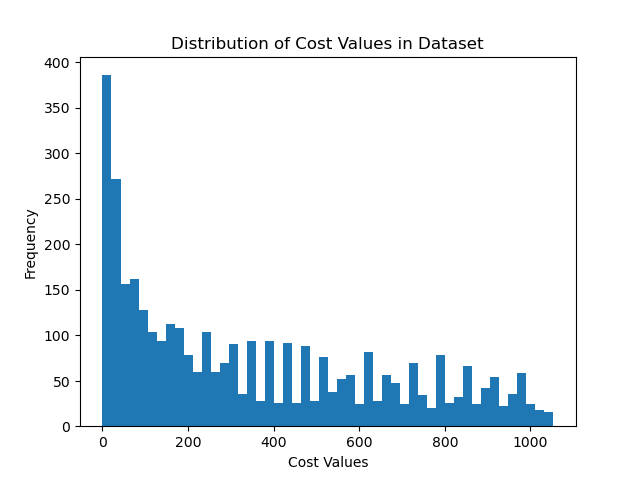
\includegraphics[width=\textwidth]{SP_cost_distr.png}
    \caption{Cost distribution of the training dataset}
  \end{subfigure}
  \begin{subfigure}[b]{0.48\textwidth}
    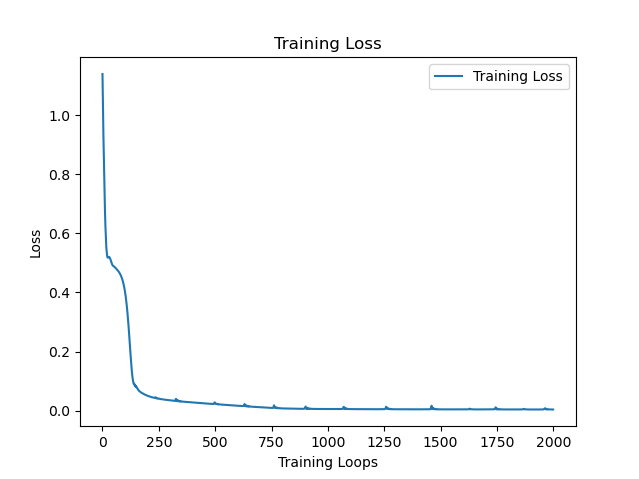
\includegraphics[width=\textwidth]{SP_loss.png}
    \caption{Loss over the training epochs}
  \end{subfigure}
  \\[0.5em]
  \begin{subfigure}[b]{0.9\textwidth}
    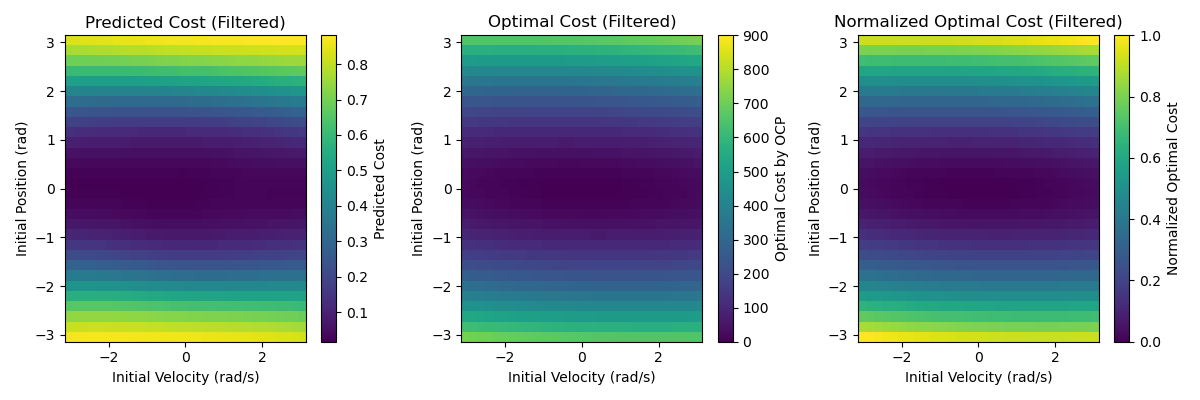
\includegraphics[width=\textwidth]{SP_colormap.png}
    \caption{Colormaps of the predicted (normalized) cost, computed cost, and normalized computed cost}
  \end{subfigure}
  \caption{Neural network training results for the single pendulum.}
  \label{fig:sp_train}
\end{figure}

\begin{figure}[htbp!]
  \centering
  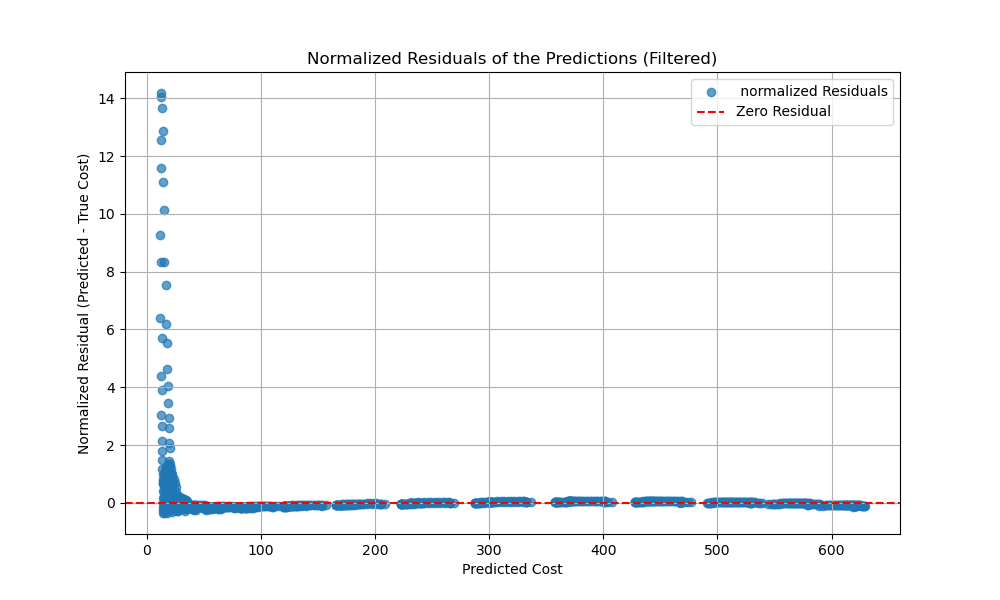
\includegraphics[width=0.7\textwidth]{SP_norm_residuals.png}
  \caption{Normalized residuals plot for the single pendulum case.}
  \label{fig:sp_res}
\end{figure}

\subsection{Open-Loop MPC Cost Comparison}

The comparison scripts \texttt{SinPendComp.py} and \texttt{SinPendComp\_multiprocess.py}
implement the three MPC formulations and compare their open-loop cost over $K=50$ random
initial states. We compute the difference between case 3 and case 2, normalized over the
long-horizon (case 2) cost, to clearly evaluate the model's performance -- overall quite good,
aside from a few outliers.

\begin{figure}[htbp!]
  \centering
  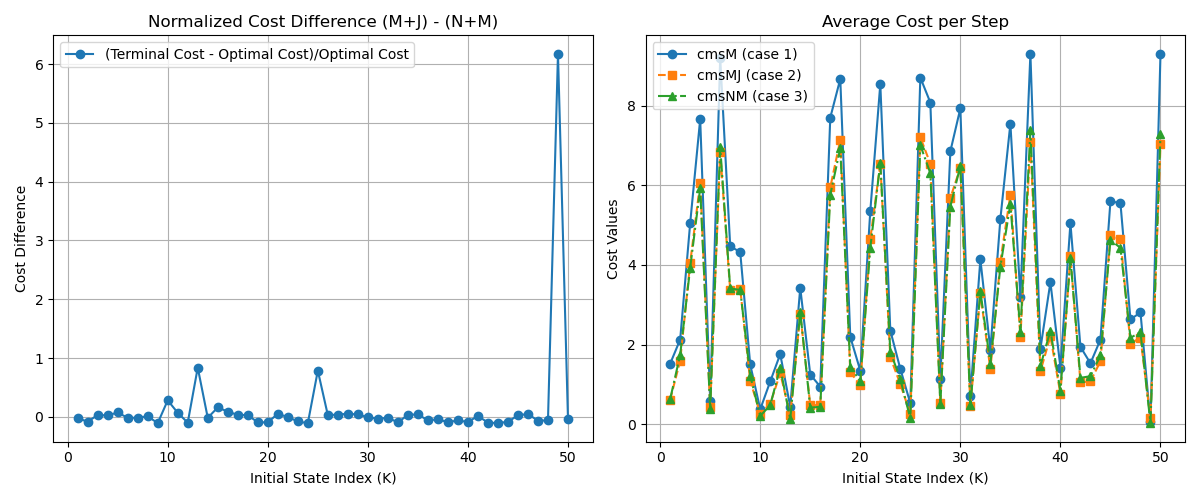
\includegraphics[width=0.95\textwidth]{SP_MPC.png}
  \caption{Left: normalized cost difference between case 3 (NN terminal) and case 2 (long
  horizon). Right: average cost per step of the three MPC formulations across $K=50$ random
  initial states.}
  \label{fig:sp_mpc}
\end{figure}

As expected, cases 2 and 3 yield similar cost values (Fig.~\ref{fig:sp_mpc}, right), and these
are consistently lower than the short-horizon case 1. This is coherent with intuition: a shorter
horizon makes the solver greedier, since it has limited predictive capability, so control actions
that look optimal in the short term can be suboptimal over a longer horizon. The lowest
achievable cost would correspond to the infinite-horizon case, globally optimal and consistent
across all MPC iterations.

\subsection{Closed-Loop MPC Trajectories}
\label{sec:sp_closed_loop}

To verify that the open-loop cost agreement above actually translates into comparable
\emph{control behaviour}, \texttt{SinPend\_MPC.py} runs all three formulations in real
receding-horizon closed loop, from the same fixed, seeded initial state $x_0 =
[0.307,\ 2.704]^T$ (rad, rad/s), for $T_{\text{sim}}=5\,$s at $\Delta t = 0.01\,$s (500 steps),
warm-starting every re-solve. $J_{\text{MAX}}$ was calibrated to $7.73$ for this run.

\begin{figure}[htbp!]
  \centering
  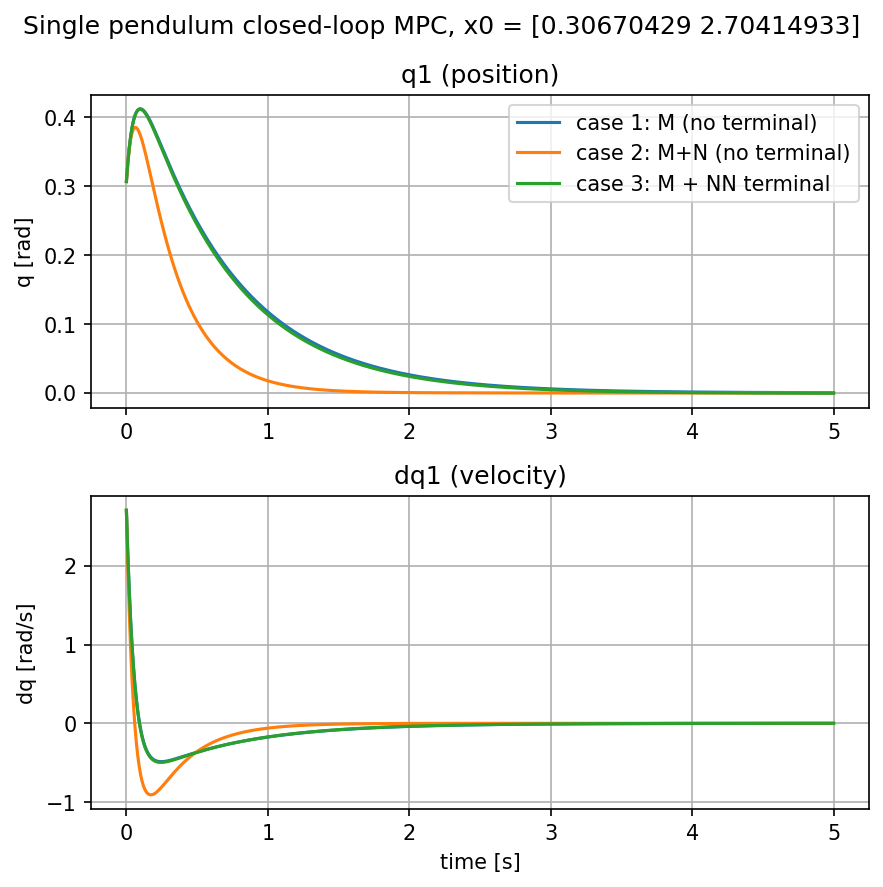
\includegraphics[width=0.75\textwidth]{SP_MPC_traj_kin.png}
  \caption{Closed-loop position $q_1$ and velocity $\dot q_1$ for the three MPC formulations,
  single pendulum.}
  \label{fig:sp_traj_kin}
\end{figure}

\begin{figure}[htbp!]
  \centering
  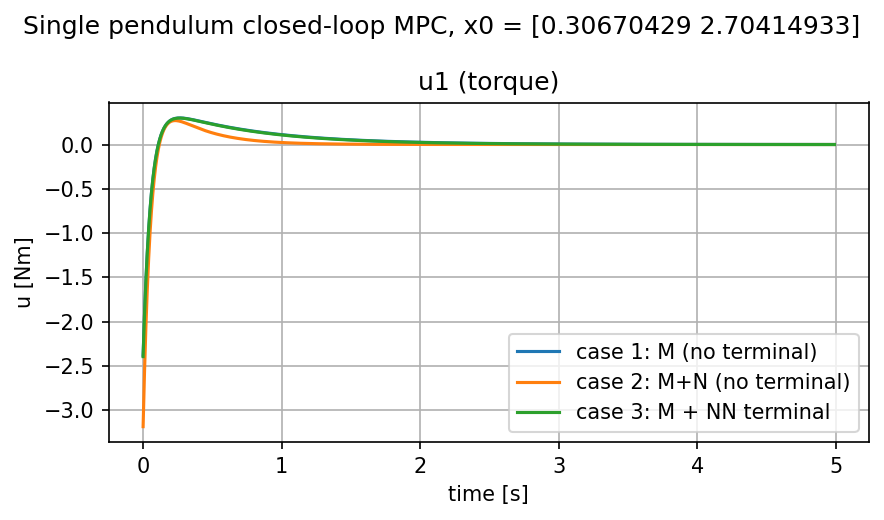
\includegraphics[width=0.75\textwidth]{SP_MPC_traj_trq.png}
  \caption{Closed-loop applied torque $u_1$ for the three MPC formulations, single pendulum.}
  \label{fig:sp_traj_trq}
\end{figure}

The closed-loop result is more nuanced than the aggregate open-loop comparison suggests.
Case 1 (short horizon, no terminal cost) and case 3 (short horizon, NN terminal cost) produce
\emph{almost indistinguishable} trajectories throughout the whole simulation, in both position/
velocity and torque -- the two curves overlap essentially everywhere in
Fig.~\ref{fig:sp_traj_kin}--\ref{fig:sp_traj_trq}. Case 2 (long horizon, no terminal cost) is
instead the visible outlier: it commands a markedly larger initial torque ($\approx -3.2\,$Nm
vs.\ $\approx -2.4\,$Nm for cases 1/3), reaches a larger negative velocity dip, and drives $q_1$
to zero noticeably faster.

This is a meaningful counterpoint to Sec.~3.4: matching the \emph{aggregate} open-loop cost
across $K=50$ random states (Fig.~\ref{fig:sp_mpc}) does not guarantee that the learned terminal
cost reproduces the long-horizon formulation's actual closed-loop \emph{policy} for a specific
initial condition. Here, the terminal-cost gradient added to the $M=20$-step Bolza cost is
evidently not strong enough to pull the short-horizon solver away from its myopic solution and
toward the more foresighted behaviour that an explicitly longer horizon (case 2) provides -- the
network correctly predicts the \emph{magnitude} of the cost-to-go on average, but that alone does
not shape the short-horizon optimizer's early control decisions the way a genuinely longer
horizon does. A larger terminal-cost weight $w_{\text{term}}$, or a network trained to also match
the \emph{gradient} of the true value function (not just its value), are natural next steps to
close this gap. (In terms of raw compute, case 3 still closed the loop in $8.1\,$s of wall-clock
time here versus $11.5\,$s for case 2 -- only a modest $1.4\times$ speed-up compared to the
double pendulum below, since the single-pendulum horizons are already small enough that the
solve-time gap between $M$ and $M{+}N$ is much less pronounced.)

\section{Double Pendulum}

We consider a 2-DOF, fully actuated, nonlinear mechanical system. As in the single-pendulum
case, the dynamics are integrated with explicit Euler; here, however, the equations of motion
are derived via the Euler--Lagrange formulation, since the actuators act directly on the
generalized coordinates, giving a straightforward computation of the generalized forces.

The full derivation is in the Maple file \texttt{double\_pend\_dynamics.mw}, where the
state-space equations are also computed. To validate the dynamics implementation, an example
(natural-response, zero-input) trajectory starting from a random initial state is shown in
Fig.~\ref{fig:dp_ex_traj}.

\begin{figure}[htbp!]
  \centering
  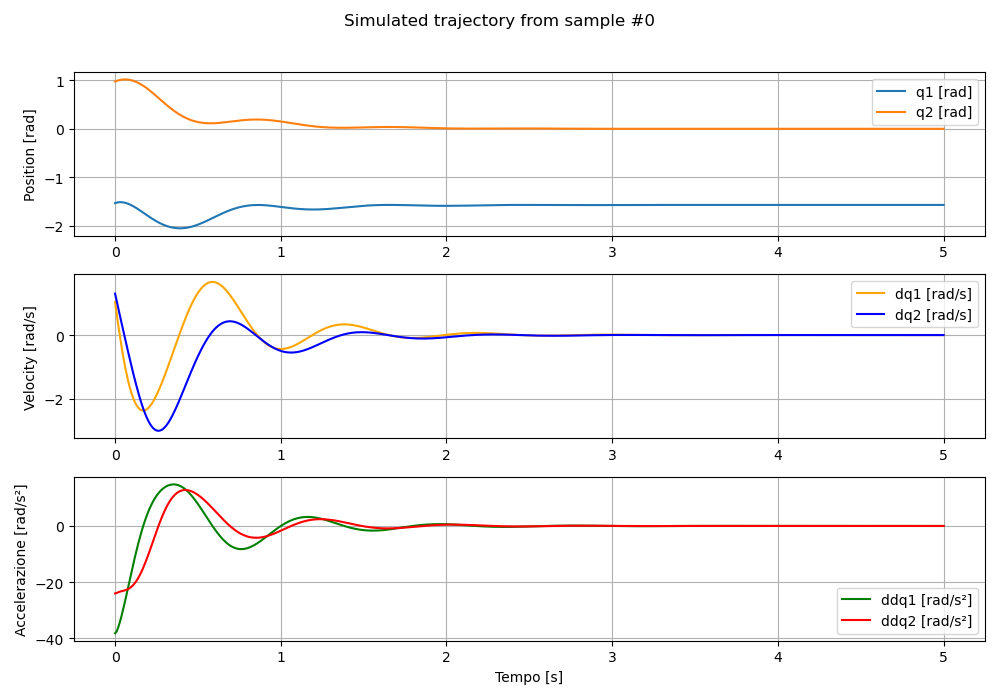
\includegraphics[width=0.75\textwidth]{DP_ex_traj.png}
  \caption{Example zero-input (natural response) trajectory, validating the double-pendulum
  dynamics implementation.}
  \label{fig:dp_ex_traj}
\end{figure}

To generate the initial conditions and compute the associated cost values for training the
neural network, a custom \texttt{Dataset} class handles both the state generation and the
parallelized cost computation. The \texttt{Pendulum} class parses the double-pendulum model
parameters (link lengths, rotational inertias about the actuated axes, distances from the
rotation axes to the centers of mass, and masses) from its URDF, including the Huygens--Steiner
contributions to the inertia terms. A new, deeper architecture, \texttt{ExtendedNeuralNetwork},
extends the capacity of the single-pendulum \texttt{NeuralNetwork} class. The training dataset
has $N_{\text{OCPs}}=3000$ points.

\subsection{Neural Network Structure}
\begin{itemize}
  \item Input layer: $x \in \mathbb{R}^4$, the initial state $x = [q_1(0), q_2(0), \dot q_1(0), \dot q_2(0)]^T$
  \item Hidden layers: 6 fully connected layers, each with 128 neurons
  \item Activation function: $\tanh$
  \item Output layer: $J(x) \in \mathbb{R}$, the predicted terminal cost
\end{itemize}

\subsection{Hyperparameters}
\begin{itemize}
  \item Learning rate: 0.009
  \item Loss function: Mean Squared Error (MSE)
  \item Training dataset size: 3000 points
  \item Input range: $\vec q \in D = [-\pi,\pi]^2$, $\dot{\vec q} \in F = [-2\pi, 2\pi]^2$
  \item Batch size: full batch
  \item Output scaling: normalized by the maximum cost in the dataset, $J_{\text{MAX}}$
  \item Training epochs: 1500
  \item Lagrange running-cost weights: $[w_p, w_v, w_a]^T = [1,\ 0.05,\ 0.03]^T$
\end{itemize}

The trained model is saved and later used to generate the scatter plot and validate performance
in \texttt{Double\_pend\_Test.py}. The final loss ($\approx 0.04$) is higher than the single-
pendulum case, consistent with the harder 4-D learning problem.

\begin{figure}[htbp!]
  \centering
  \begin{subfigure}[b]{0.48\textwidth}
    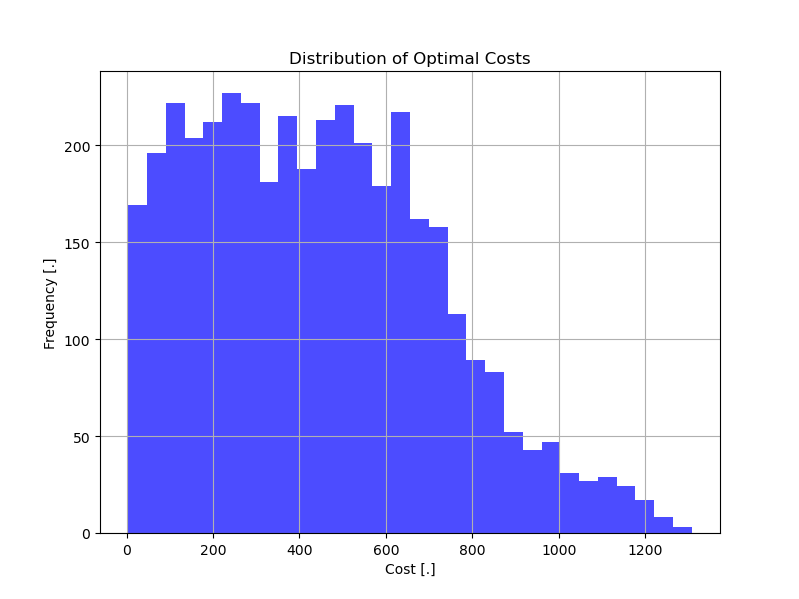
\includegraphics[width=\textwidth]{DP_cost_dist.png}
    \caption{Cost distribution of the training dataset}
  \end{subfigure}
  \begin{subfigure}[b]{0.48\textwidth}
    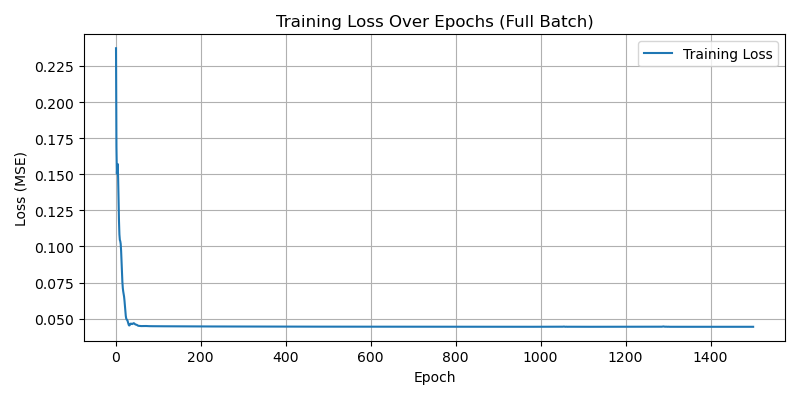
\includegraphics[width=\textwidth]{DP_loss.png}
    \caption{Loss over the training epochs}
  \end{subfigure}
  \\[0.5em]
  \begin{subfigure}[b]{0.48\textwidth}
    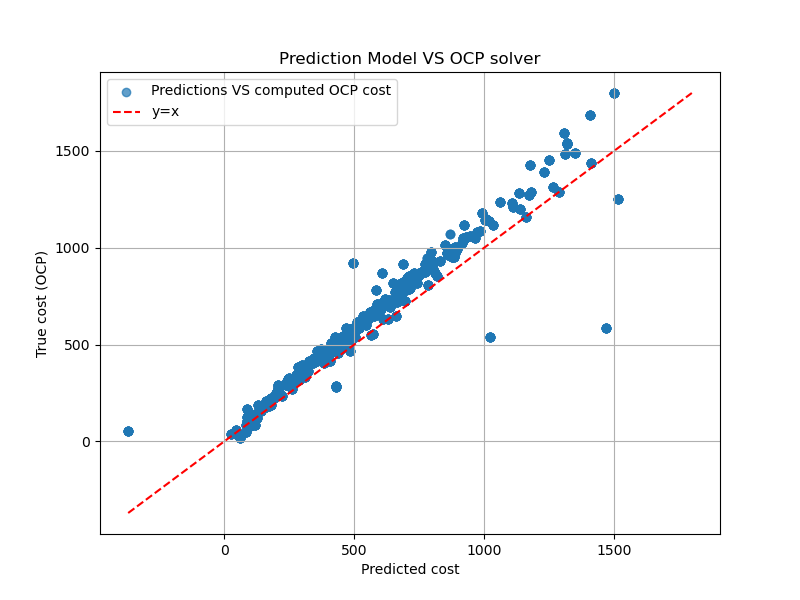
\includegraphics[width=\textwidth]{DP_scatter.png}
    \caption{Scatter plot: predicted vs.\ computed cost}
  \end{subfigure}
  \begin{subfigure}[b]{0.48\textwidth}
    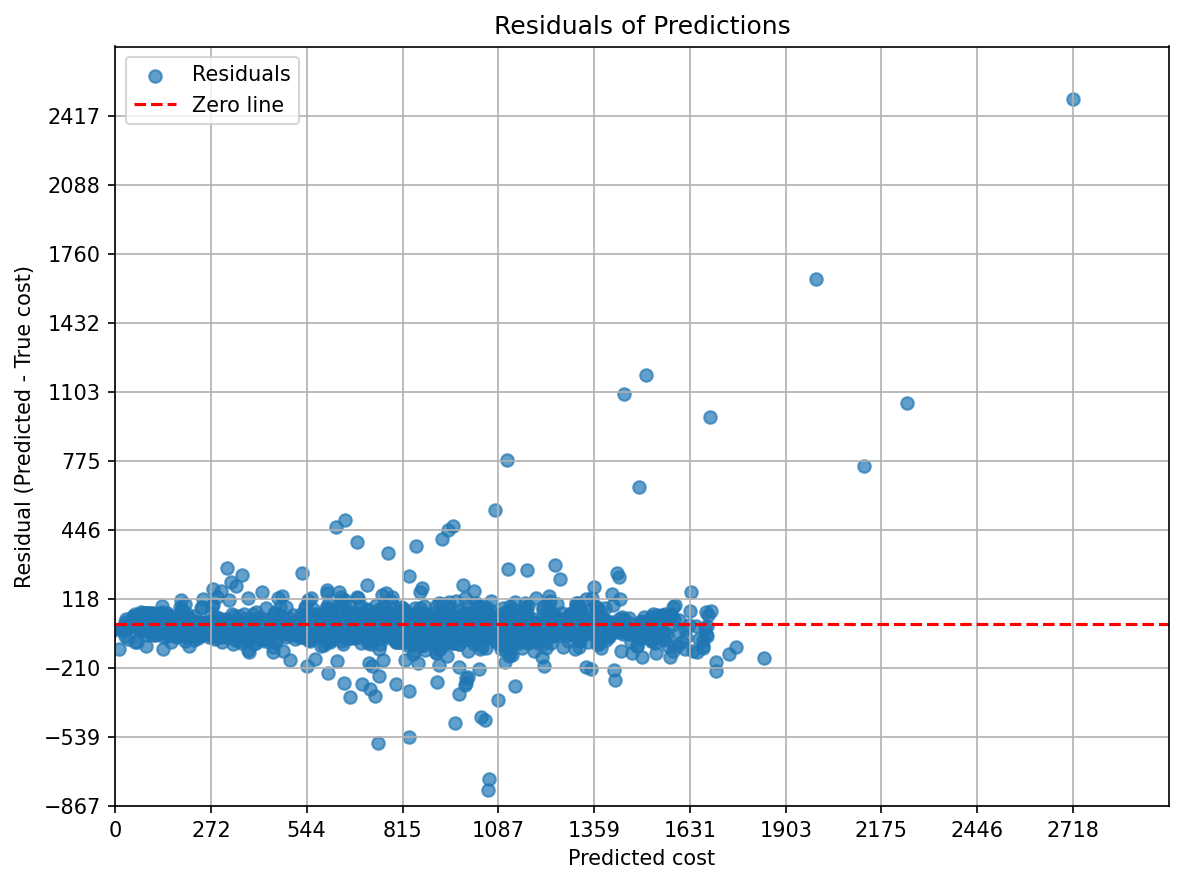
\includegraphics[width=\textwidth]{DP_residuals.png}
    \caption{Residuals plot}
  \end{subfigure}
  \caption{Neural network training results for the double pendulum.}
  \label{fig:dp_train}
\end{figure}

\subsection{Open-Loop MPC Cost Comparison}

\texttt{Double\_pend\_comp.py} and \texttt{Double\_pend\_comp\_multi.py} implement the same
three-case comparison as the single-pendulum case.

\begin{figure}[htbp!]
  \centering
  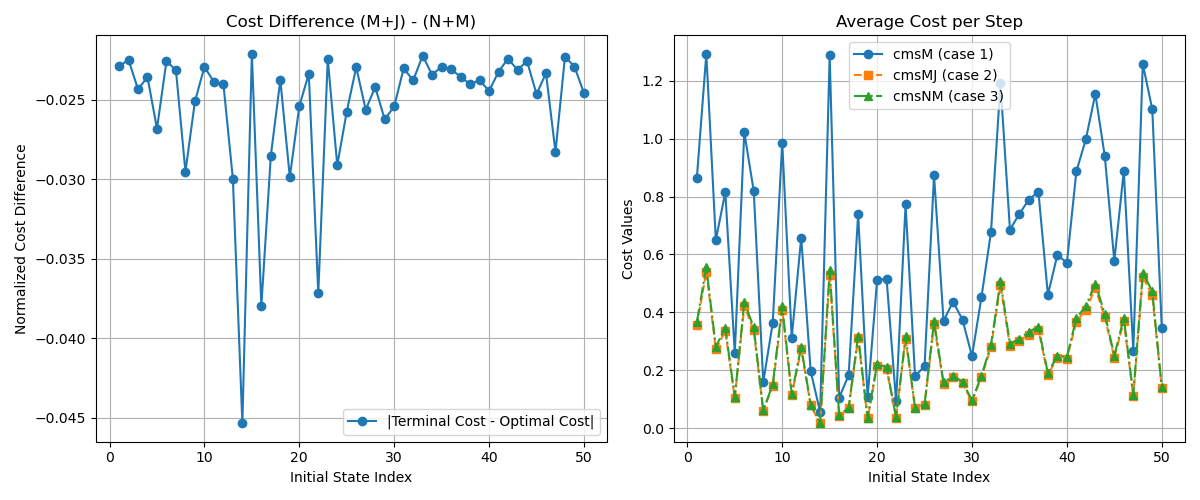
\includegraphics[width=0.95\textwidth]{DP_MPC.png}
  \caption{Left: normalized cost difference between case 3 (NN terminal) and case 2 (long
  horizon). Right: average cost per step of the three MPC formulations, double pendulum.}
  \label{fig:dp_mpc}
\end{figure}

\subsection{Closed-Loop MPC Trajectories}
\label{sec:dp_closed_loop}

\texttt{Double\_pend\_MPC.py} runs the same closed-loop experiment as
Sec.~\ref{sec:sp_closed_loop}, for $T_{\text{sim}}=5\,$s at $\Delta t=0.01\,$s, from the same
seeded initial-state distribution, with horizons $M=70$, $N=200$ ($M+N=270$).

\begin{figure}[htbp!]
  \centering
  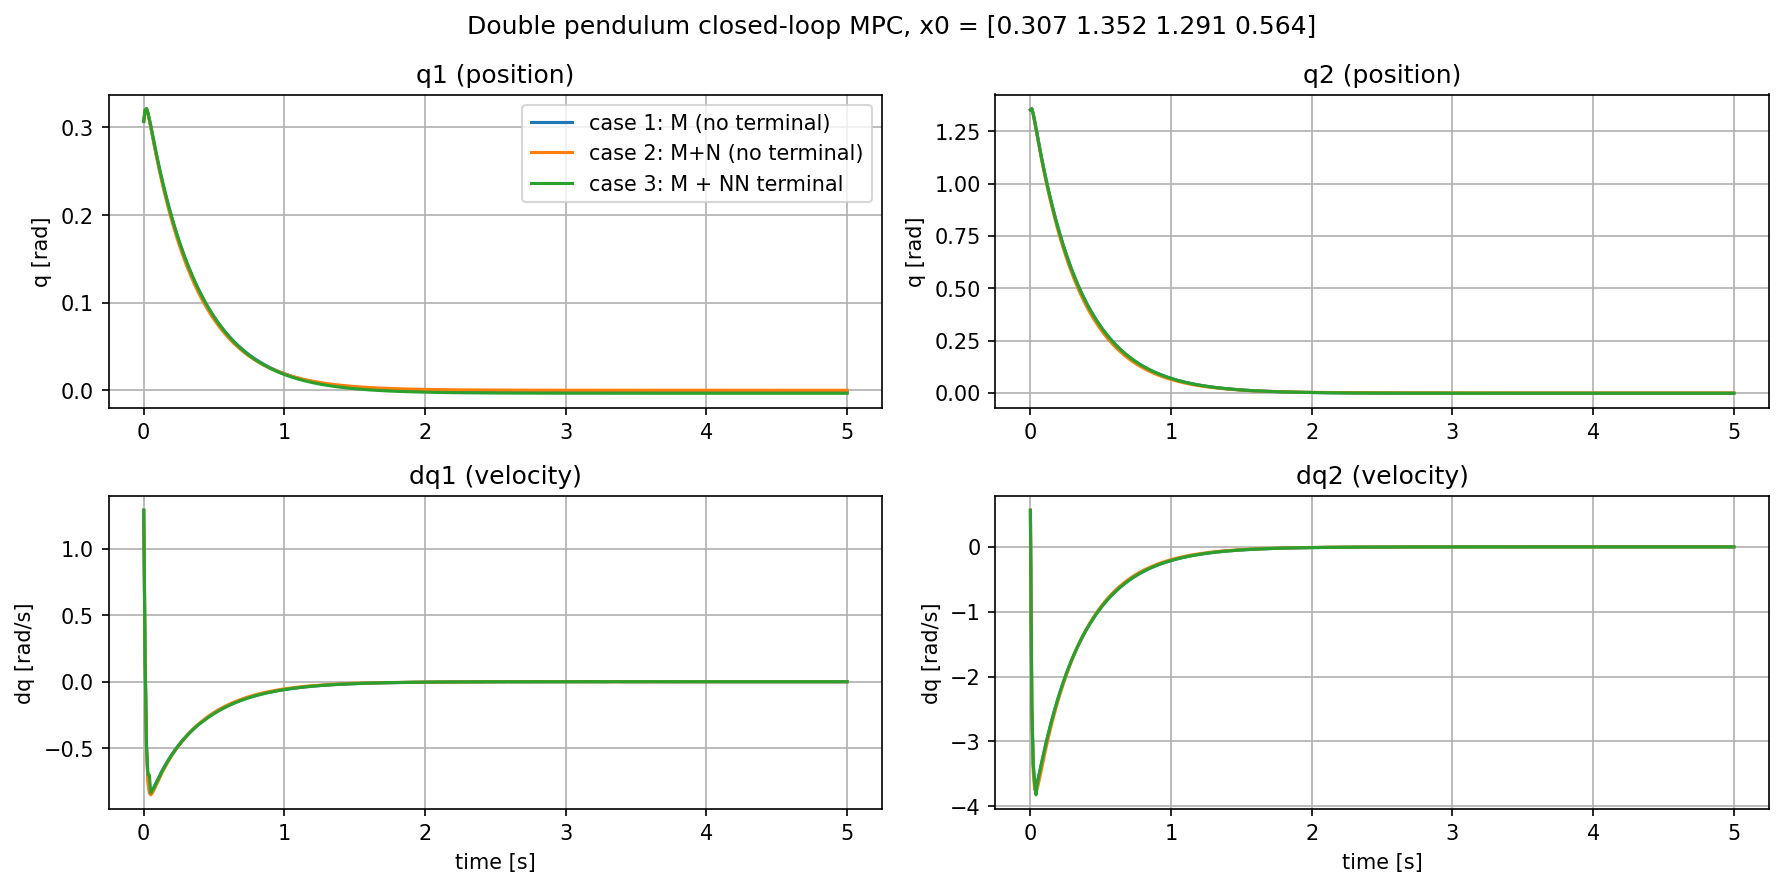
\includegraphics[width=0.95\textwidth]{DP_MPC_traj_kin.png}
  \caption{Closed-loop positions $q_1, q_2$ and velocities $\dot q_1, \dot q_2$ for the three MPC
  formulations, double pendulum.}
  \label{fig:dp_traj_kin}
\end{figure}

\begin{figure}[htbp!]
  \centering
  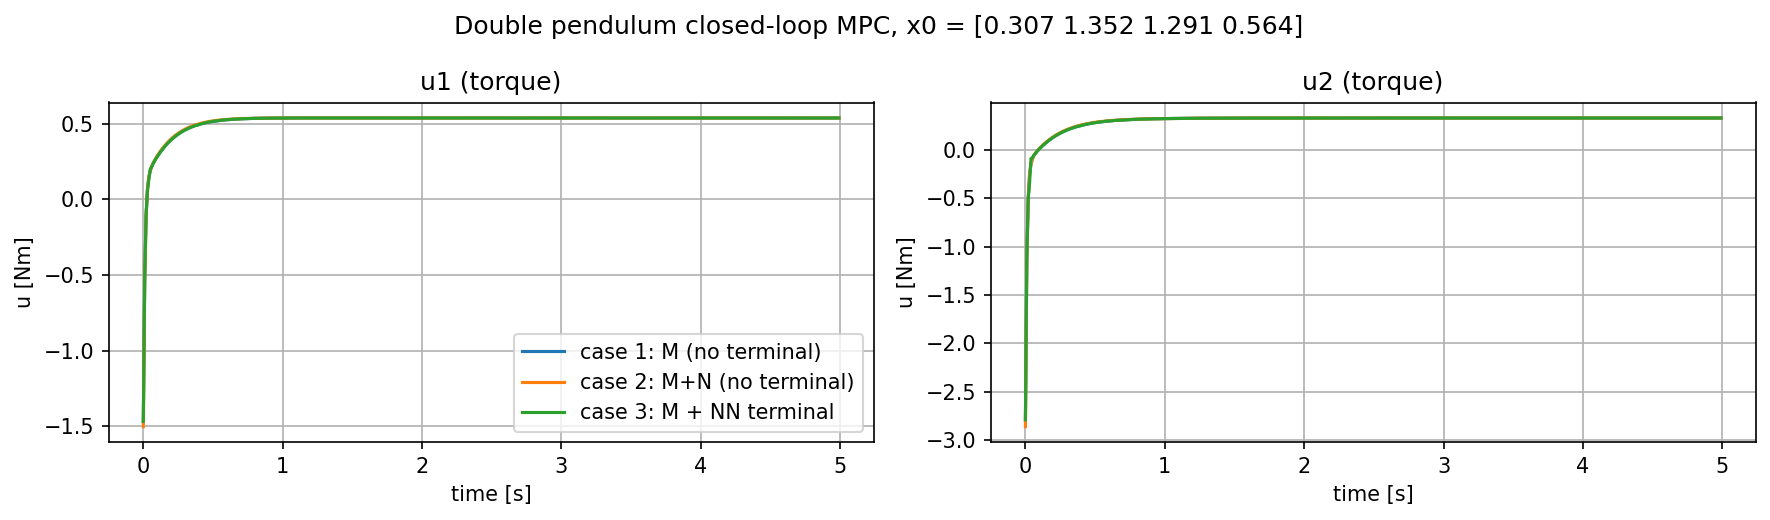
\includegraphics[width=0.95\textwidth]{DP_MPC_traj_trq.png}
  \caption{Closed-loop applied torques $u_1, u_2$ for the three MPC formulations, double
  pendulum.}
  \label{fig:dp_traj_trq}
\end{figure}

Here the picture is markedly different from the single-pendulum case: all three formulations
produce trajectories that are visually indistinguishable across the full $5\,$s window, in
position, velocity, \emph{and} torque, for both joints (Figs.~\ref{fig:dp_traj_kin},
\ref{fig:dp_traj_trq}). Unlike Sec.~\ref{sec:sp_closed_loop}, case 1 (myopic, $M=70$ steps
$=0.7\,$s lookahead) does not visibly diverge from cases 2/3 here. A likely explanation is that,
for this particular seeded initial state (a damped settling toward the origin, with no swing-up
or actuation-limit maneuvering involved), a $0.7\,$s lookahead is already long enough that the
greedy and far-sighted policies agree -- the double pendulum's $M$ is proportionally similar to
the single pendulum's ($M/(M{+}N) \approx 26\%$ vs.\ $20\%$), but in absolute time it is $3.5\times$
longer, which matters more for how much of the settling transient the controller can already
``see''.

When the three formulations do agree this closely, the value of the terminal cost is not
visible in \emph{trajectory shape} but in \emph{computational cost}: in this run, case 2
($N_{\text{pred}}=270$) took $178.9\,$s of wall-clock time for the closed-loop simulation, while
case 3 ($N_{\text{pred}}=70$, with the learned terminal cost, $J_{\text{MAX}}=0.599$) took only
$51.7\,$s -- a $3.46\times$ speed-up for control that is, for this initial condition, essentially
identical. This is the cleanest demonstration in this report of the method's actual payoff:
the same closed-loop behaviour at a fraction of the per-step solve cost. Whether this speed-up
comes with a trajectory-quality cost for \emph{other} initial states -- particularly ones nearer
the training domain's high-cost boundary, where Fig.~\ref{fig:dp_train}d shows the network is
least accurate -- is a natural extension of this experiment (evaluating several seeded $x_0$
rather than one, as already done for the open-loop comparison in Fig.~\ref{fig:dp_mpc}).

\section{Discussion and Final Remarks}

As already observed for the single pendulum, the (extended) neural-network architecture predicts
the terminal cost function accurately within the training domain in both systems, enabling
effective integration in an MPC framework -- Figs.~\ref{fig:sp_mpc} and \ref{fig:dp_mpc} confirm
this in aggregate, open-loop terms. The double-pendulum learning task is harder, owing to the
higher-dimensional input and stronger nonlinearity of both dynamics and cost function; this shows
up in the residuals plot (Fig.~\ref{fig:dp_train}d), where larger prediction errors appear in
specific regions of the input space, likely those with steep cost gradients or near the domain
boundaries -- consistent with the higher final training loss ($\approx 0.04$ vs.\ $\approx 0.002$
for the single pendulum).

\paragraph{On the high-cost residual drift.} Looking more closely at where those larger errors
concentrate (Fig.~\ref{fig:dp_train}d), two compounding, and largely untested, causes are worth
flagging beyond activation saturation. First, the training-set cost distribution
(Fig.~\ref{fig:dp_train}a) is heavily skewed: most of the 3000 samples cluster at low-to-mid cost,
with only a thin tail reaching the highest values -- the network simply sees far fewer examples in
exactly the region where it needs to be most accurate. Second, and less obvious, the ``ground
truth'' labels themselves may be noisier there: at high $\dot q$ (sampled up to $\pm 2\pi$), the
double pendulum's cost landscape is more strongly nonlinear and plausibly multi-modal, so IPOPT
reporting \texttt{Solve\_Succeeded} does not guarantee convergence to the \emph{global} optimum --
\texttt{Double\_pend\_training.py}'s \texttt{Dataset} class filters outright failed solves, but not
solves that converged to a local optimum, which would inject inconsistent labels precisely in the
high-cost tail and could show up as drift rather than pure variance. Separately, it is worth noting
that \texttt{SinPendTrain.py} already \emph{attempts} a fix for the first issue -- a per-sample
loss weight that upweights high-cost training points -- but as written it does not do what it
intends: \texttt{nn.MSELoss()} defaults to \texttt{reduction='mean'}, which collapses the loss to a
scalar \emph{before} the per-sample \texttt{weights} tensor is multiplied in, so the result is only
a constant rescaling of the whole loss, not an actual per-sample reweighting (that would require
\texttt{nn.MSELoss(reduction='none')} first). Fixing that and porting it to the double-pendulum
training script, combined with auditing high-cost samples for local-minima labels, are the two
most promising and cheapest next steps -- ahead of, e.g., switching activations -- since they
target the likely root cause (data quantity/quality in the tail) rather than the symptom.

The closed-loop experiments added in this revision (Secs.~\ref{sec:sp_closed_loop},
\ref{sec:dp_closed_loop}) are the central addition of this report: they test the learned
terminal cost inside an actual running controller, not just as a one-shot cost predictor. The
central payoff the network is meant to deliver -- case 3 reproducing case 2's trajectory quality
at case 1's per-step computational cost -- is not automatic just because case 3 matches case 2 in
\emph{aggregate open-loop cost}; the single-pendulum result in Sec.~\ref{sec:sp_closed_loop} is a
concrete instance where it does not hold for a specific initial condition, which is exactly the
kind of failure mode that an open-loop-only evaluation cannot reveal.

\paragraph{Possible improvements.} From the colormap plot (Fig.~\ref{fig:sp_train}c) and the
double-pendulum residuals (Fig.~\ref{fig:dp_train}d), the network struggles most near the
boundaries of the training domain, precisely where the cost is highest and its gradient is
steepest -- a harder regime for a fixed sampling density, and one where a saturating activation
like $\tanh$ compresses large output values, since $\tanh: \mathbb{R} \to (-1,1)$. Switching to a
non-saturating (or less saturating) activation such as ReLU, Leaky ReLU, Swish, or ELU could help
the network better approximate large cost values in high-gradient regions. Non-uniform sampling
(denser near the boundaries) and normalizing cost values before training could also help. More
expressive architectures (residual or attention-based networks) could better capture sharp
transitions in the cost landscape. Finally, the closed-loop analysis above suggests that
\emph{matching the value function alone is not sufficient} for the terminal cost to reproduce the
long-horizon closed-loop policy: increasing $w_{\text{term}}$, or training the network against
the value function's \emph{gradient} in addition to its value (e.g., via a Sobolev-training loss),
are promising directions to make the terminal cost actively steer the short-horizon solver, not
just match its expected cost.

\end{document}
